\documentclass{article}
\usepackage{comment}
\usepackage{graphicx}
\usepackage[utf8]{inputenc}
\usepackage[english]{babel}

\begin{document}

\title{Using wavelengths outside of the Telecom spectrum}
\author{Stefan Plug\\Remy de Boer}
\date{\today}
\maketitle

\begin{comment}
\begin{tabular}{|c|c|c|}
\hline 
Version number & Date & Comment \\ 
\hline 
0.1 & 03-01-2013 & Start of of document \\ 
\hline 
\end{tabular} 
\end{comment}

\tableofcontents
\newpage

\section{Preface}
\newpage
\section{Summary}
\newpage
\section{Research question}
It is common practice today to use Wavelength Division Multiplexing, WDM, devices on network links to increase the total amount of bandwidth that a single optical network link can carry. The WDM accomplishes this by assigning each input data stream its own unique light wavelength channel, $\lambda$. 
Not every wavelength is suitable for heavy traffic usage because of the physical characteristics of these channels. Our hypothesis is that these channels could be used for lower speed applications such as monitoring and out of band management.

To test our hypothesis we will look at the possibilities of the unused wavelengths outside of the Telecom spectrum.
The main research question will be as follows:
\begin{quote}
\textit{
What applications can the unused wavelengths outside of the Telecom spectrum be used for?
}
\end{quote}

It is important to be able to have an active monitoring system in place which can send out warnings when it detects either degradation of the link over time or a sudden change in the links characteristics, for example when someone places a tap on the link. 

To help us understand how we can effectively monitor an optical link we will ask the following sub-question:
\begin{quote}
\textit{
What optical link characteristics should we monitor?
}
\end{quote}

It could happen that the main traffic interface on a switch shuts down which could potentially shut down that section of the network.
It would be good to have a separate out of band network link up on another interface which could be used to still manage that device.

During this project we will focus on link monitoring and out of band management, but other usages may arise during our research.
If this should happen we shall try to document them.

\newpage
\section{Fibre Technology}
In this chapter we will elaborate on some of the used technology and techniques used for this research project.
\subsection{Fibreglass cables}
When using fibreglass networks, multiple types of fibreglass cables are used.
The two main categories used in computer networking are multi-mode and single-mode cables.
Multi-mode cables differ from single-mode cables as they consist of a larger core, which allows for easier connections and cheaper light sources such as LEDs. \cite{Fundamentals:2008}
For our projects we are focussing on single-mode cables, as these are the cables used with Wavelength Division Multiplexing (WDM).

\subsection{Wavelength division multiplexing}
Wavelength division multiplexing is a technique used to send multiple independent signals across the same fibre.
WDM works by combining optical signals of different wavelengths into a single fibre to increase the maximum bandwidth of a fibreglass cabl, thus allowing multiple completely separate connections to run along a single fibre cablee.
On either end of the single fibre cable, the signals are split into individual fibre cables and connected to their final destinations.

This ITU-T standard shows us that the 1625nm channel which resides at the beginning of the L-band is not officially supported by several of the single-mode optical cable standards as show in table \ref{tab:single-mode_types}.

\begin{table}[h]
\centering
\label{tab:single-mode_types}
\caption{ITU-T Single-mode cable standards}
\begin{tabular}{|c|c|c|}
\hline 
ITU-T code & Wavelength coverage\\ 
\hline 
G.652.A & O and C bands \\ 
\hline
G.652.B & O and C+L bands \\
\hline
G.652.C & From O to C bands \\
\hline
G.652.D & From O to L bands \\
\hline
\end{tabular} 
\end{table}

The cables which do not officially support the 1625nm channel are expected to generate a higher attenuation effect. Although we will not try to test this effect for all the different kinds of fibre, we should keep this in mind during testing.

\newpage
\section{Proof of Concept}
To test our hypotheses we were provided with two Inteno XG6746\cite{Inteno:XG6746} switches by our sponsors. It is in the interest of our sponsor that we can use this relatively cheap equipment instead of specialised, and usually more expensive OTDR equipment. The Inteno XG6746 switches have one modular SFP fiber optic port in which we can place our testing optics. 

We would like the fibre optic switches to communicate with each other so they can exchange statistics about their fibre optics and use these statistics to create MRTG\cite{MRTG:MRTG} graphs that could show interesting trends which might be an indicator of fibre degradation over time.

The Inteno XG6746 runs on the software image \texttt{XG6746\_4.02ITT24.01\_20121022}. Because of the closed nature of the software we were not able to directly install programs or scripts which we needed to generate traffic on the fibre link directly.
In the limited time we were allotted for this project we were not able to get any other OS to work. The current software does allow us to read out essential information such as Rx and Tx Decibels of the optic via SNMP.

To still be able to run diagnostic tests we decided to attach a Raspberry Pi to to the switch via Ethernet which can both generate traffic and do periodic polling via SNMP.
Ideally all the functions performed by the Raspberry Pi would be integrated into the Inteno XG6746, however to simplify matters we chose to use a Raspberry Pi as it boasts a full-fledged Linux environment, Raspbian\cite{raspbian:raspbian}.

For our tests we will use 1625nm optics. for comparison we will also run the same tests on ....nm optics. To validate our test-network itself we will also run similar tests on specialised OTDR equipment using the same optics.

\subsection{Testing equipment}

PUT ALL HARDWARE WE USED IN THIS CHAPTER INCLUDING ALL OPTICS AND OTDRs
\begin{itemize}
\item Inteno XG6746 \cite{Inteno:XG6746}
\begin{itemize}
\item Broadcom 6338
\item Marvell 88E6161
\item 8 MB Flash
\item 32 MB RAM
\end{itemize}

\item Raspberry Pi - Model B

\item Optics:
\begin{itemize}
\item SFP
\item EOptolink
\item EOLS-1603-29SD
\item 1625nm
\end{itemize}
\end{itemize}

\subsection{Test network}
\begin{figure}[h]
\centerline{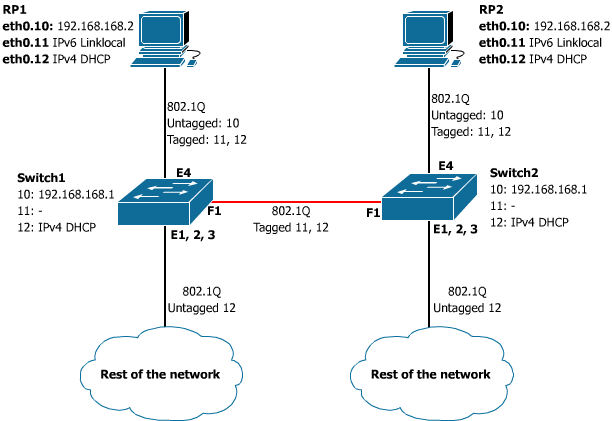
\includegraphics[scale=0.4]{images/PoC_all.png}}
\caption{Network diagram of the test setup}
\label{fig:poc_all}
\end{figure}

Figure~\ref{fig:poc_all} on page~\pageref{fig:poc_all} shows our test setup.
It is important to note that we use 3 separate VLANs. 

\begin{figure}[h]
\centerline{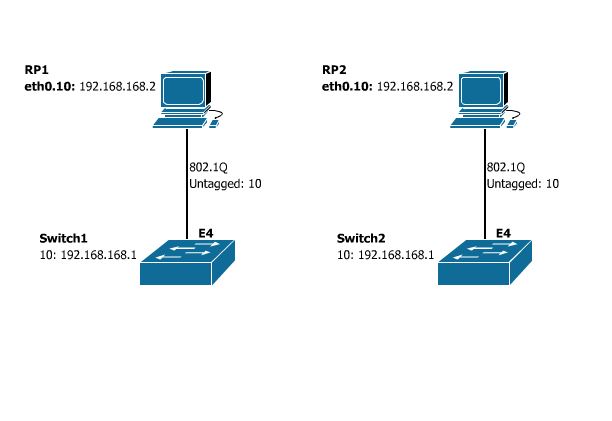
\includegraphics[scale=0.4, trim = 0mm 50mm 0mm 0mm]{images/PoC_10.png}}
\caption{Network diagram of VLAN-10}
\label{fig:poc_10}
\end{figure}

The purpose of \texttt{VLAN-10} as show in figure~\ref{fig:poc_10} on page~\pageref{fig:poc_10} is to create a single unit out of 1 Raspberry Pi and 1 monitored switch. This way \texttt{RP1} will only monitor \texttt{Switch1} although \texttt{Switch2} uses the same default IPv4 address as \texttt{Switch1}. In the ideal situation where the \texttt{RP\#} and \texttt{Switch\#} would be combined into 1 device this VLAN would be obsolete.

\begin{figure}[h]
\centerline{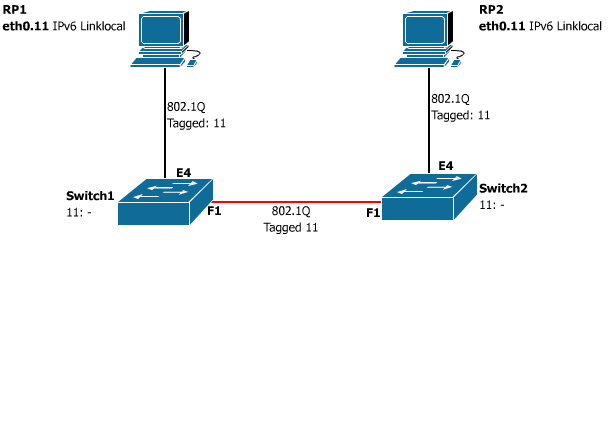
\includegraphics[scale=0.4, trim = 0mm 70mm 0mm 0mm]{images/PoC_11.png}}
\caption{Network diagram of VLAN-11}
\label{fig:poc_11}
\end{figure}

Figure~\ref{fig:poc_11} on page~\pageref{fig:poc_11} shows \texttt{VLAN-11} which is used to exchange data between 2 \texttt{RP\#} devices. This VLAN creates a group of 2 \texttt{VLAN-10} units using the fiber optics in port \texttt{F1} on \texttt{Switch\#}. The \texttt{RP\#} devices use an IPv6 Link local address, this is done so there is no need to manually configure an IP address when 2  \texttt{VLAN-10} units are connected to each other. The 2 RPs can discover each other by sending a ping to IPv6 multicast address \texttt{FF02::1} to which all IPv6 linklocal hosts should listen and reply too\cite{ietf:rfc4291}. After the RP knows the IPv6 address of a potential neighbour it will do a simple check to see if that neighbour is indeed our polling partner and not some rouge computer. It will do this by sending a SHA256 hash of a common pre-shared password plus its own linklocal IPv6 address which should protect against a simple re-play attack.

\begin{figure}[h]
\centerline{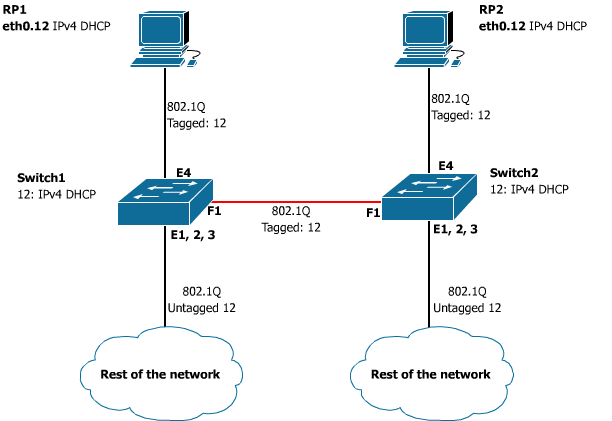
\includegraphics[scale=0.4, trim = 0mm 0mm 0mm 0mm]{images/PoC_12.png}}
\caption{Network diagram of VLAN-12}
\label{fig:poc_12}
\end{figure}
Figure~\ref{fig:poc_12} on page~\pageref{fig:poc_12} shows \texttt{VLAN-12} which is used to connect our devices to the rest of the network and thus might be used for out-of-band management.

\newpage
\section{tests}
We would like to find out if we can use the 1625nm wavelength to do reliable tests of a fibre. we can do this by 





\newpage
\section{Conclusion}
\bibliographystyle{plain}
\bibliography{bibliography}

\end{document}